% ---------------------------------------------------------------------
\subsection{Inversao de Matrizes}\label{subsec:inversao}
% ---------------------------------------------------------------------

\subsubsection{Decomposicao de Cholesky}


% ---------------------------------------------------------------------
% SEPARAÇÃO (2026-11-04): conceitos trazidos do rascunho (Parte 1.5) e de
%   METODOLOGIA/requisitos-tempo.tex (vazão, latência e II).
% ---------------------------------------------------------------------
\subsubsection{\textcolor{red}{Representação em ponto fixo}}\label{subsubsec:ponto-fixo}
\textcolor{red}{Em hardware, os números costumam ser representados em ponto fixo. No Vitis HLS, o tipo \texttt{ap\_fixed}$\langle W, I\rangle$ tem $W$ bits no total, dos quais $I$ são da parte inteira \cite[p.~73--74]{kastner-hls}. A parte fracionária tem $F = W - I$ bits. Neste trabalho, o formato é escrito como $\langle W, I\rangle$.}

\textcolor{red}{Quando um valor não cabe na parte inteira, ocorre um estouro (\textit{overflow}). Uma forma comum de tratá-lo é descartar os bits mais significativos, o que se chama \textit{wrapping} \cite[p.~70]{kastner-hls}. Em complemento de dois, isso pode até trocar o sinal do número \cite[p.~71]{kastner-hls}. Quando um valor não cabe na parte fracionária, ele precisa ser arredondado \cite[p.~71]{kastner-hls}. Descartar os bits extras arredonda em direção a $-\infty$. Outras formas arredondam em direção a $+\infty$, em direção a zero, para longe de zero, ou para o valor mais próximo, com o empate indo para o valor par \cite[p.~71]{kastner-hls}.}

\textcolor{red}{O tipo \texttt{ap\_fixed} tem 7 modos de quantização e 5 modos de estouro, o que dá 35 combinações. A Tabela~\ref{tab:modos-apfixed} descreve cada um.} % TODO FONTE: UG1399.

\begin{table}[htbp]
\caption{\textcolor{red}{Modos de quantização e de estouro do tipo \texttt{ap\_fixed}.}}
\label{tab:modos-apfixed}
\centering
\footnotesize
\begin{tabular}{p{2.6cm}p{11cm}}
\toprule
Modo & Comportamento \\
\midrule
\multicolumn{2}{l}{\textit{Quantização (afeta os bits fracionários)}} \\
\texttt{AP\_TRN}       & Descarta os bits menos significativos. Arredonda em direção a $-\infty$. \\
\texttt{AP\_TRN\_ZERO} & Arredonda em direção a zero. Para números positivos, é igual ao \texttt{AP\_TRN}. \\
\texttt{AP\_RND}       & Arredonda para o valor mais próximo. No empate, arredonda em direção a $+\infty$. \\
\texttt{AP\_RND\_ZERO} & Arredonda para o valor mais próximo. No empate, arredonda em direção a zero. \\
\texttt{AP\_RND\_MIN\_INF} & Arredonda para o valor mais próximo. No empate, arredonda em direção a $-\infty$. \\
\texttt{AP\_RND\_INF}  & Arredonda para o valor mais próximo. No empate, afasta-se de zero. \\
\texttt{AP\_RND\_CONV} & Arredonda para o valor mais próximo. No empate, vai para o valor par. \\
\midrule
\multicolumn{2}{l}{\textit{Estouro (afeta os bits inteiros)}} \\
\texttt{AP\_SAT}       & Satura no maior ou no menor valor representável. \\
\texttt{AP\_SAT\_ZERO} & Em caso de estouro, o resultado vira zero. \\
\texttt{AP\_SAT\_SYM}  & Satura de forma simétrica: os limites positivo e negativo têm o mesmo módulo. \\
\texttt{AP\_WRAP}      & Descarta os bits mais significativos que não cabem (estouro em complemento de dois). \\
\texttt{AP\_WRAP\_SM}  & Faz o mesmo descarte, mas em sinal e magnitude. \\
\bottomrule
\end{tabular}
\legend{\textcolor{red}{Fonte: TODO (UG1399).}}
\end{table}
% ORIGEM: Análise bits.md, corrigido (AP_TRN_ZERO). Frases de custo de hardware dos
%   modos ficaram fora (sem fonte). Kastner et al. só tratam os conceitos, não os nomes
%   dos modos; para os nomes, a UG1399.

\subsubsection{\textcolor{red}{Latência, intervalo e vazão}}\label{subsubsec:latencia-intervalo}
\textcolor{red}{Em síntese de alto nível, uma tarefa é uma chamada de função. A latência da tarefa é o tempo entre o início e o fim de uma tarefa. O intervalo da tarefa é o tempo entre o início de uma tarefa e o início da seguinte \cite[p.~20]{kastner-hls}. Em um circuito com \textit{pipeline}, uma nova tarefa pode começar antes de a anterior terminar. Assim, o intervalo pode ser menor que a latência \cite[p.~21]{kastner-hls}. O intervalo entre dois dados que entram no \textit{pipeline} é chamado de intervalo de iniciação (II, \textit{Initiation Interval}) \cite[p.~21]{kastner-hls}.}

\textcolor{red}{No começo, o \textit{pipeline} está vazio, e só os primeiros estágios trabalham. O tempo até todos os estágios ficarem ocupados é o tempo de enchimento. No fim, o \textit{pipeline} também precisa esvaziar. Esse custo fixo pesa mais quando há poucas iterações \cite[pp.~114 e 146]{kastner-hls}.}

\textcolor{red}{Em uma sequência de tarefas, a primeira termina depois da latência $L$, e cada uma das seguintes, um intervalo $I$ depois da anterior. Assim, $n$ tarefas terminam em}
\begin{equation}\label{eq:fim-tarefas}
\textcolor{red}{t_n = L + (n-1)\, I.}
\end{equation}
% MOVIDO (2026-11-06) de METODOLOGIA/arquiteturas-hardware.tex (subseção "Pipeline e tempo de
%   enchimento"). Enchimento: redação própria; o livro não tem frase literal. Passagens:
%   p. 114 ("Once the pipeline is full, all four subfunctions are executing concurrently"),
%   p. 146 (esvaziamento; custo fixo em laços curtos). A Eq. sai das definições de latência
%   e intervalo (p. 20-21) e do exemplo da p. 45 (4 + (11-1)·1 = 14 ciclos).

\textcolor{red}{Muitas ferramentas chamam o intervalo de vazão (\textit{throughput}). Um intervalo maior quer dizer menos tarefas por unidade de tempo, ou seja, uma vazão menor \cite[p.~22]{kastner-hls}. Neste trabalho, a vazão é medida pelo intervalo entre inversões, e a latência é o tempo de uma inversão.}
% FONTE: Kastner et al. 2018 (books/Parallel Programming for FPGAs.pdf): p. 20
%   (task latency/interval), Fig. 1.7 p. 21 (pipelined: interval 1 < latency 10),
%   p. 21 (initiation interval), p. 22 (ferramentas chamam o intervalo de throughput).
% A CONFERIR: páginas contadas pelo PDF (páginas impressas iguais às do PDF neste livro).


\subsubsection{\textcolor{red}{Pipeline de tarefas}}\label{subsubsec:pipeline-tarefas}
\textcolor{red}{Uma tarefa pode ser dividida em etapas. No \textit{pipeline} de tarefas, as etapas trabalham ao mesmo tempo, cada uma em um dado diferente. Assim, a tarefa seguinte começa quando a anterior termina a primeira etapa. Em HLS, isso é feito com a diretiva \texttt{dataflow}, e cada etapa vira um processo separado. O intervalo do conjunto nunca é menor que o intervalo da etapa mais lenta \cite[pp.~113--115]{kastner-hls}.}
% FONTE: Kastner p. 113 ("different stages of the algorithm are operating on different data
%   sets. This optimization, called task pipelining is enabled using the dataflow directive"),
%   p. 114 (a segunda tarefa começa depois que a primeira termina a primeira função;
%   "pipeline stages (often called processes)"), p. 115 ("the achieved interval for the
%   overall pipeline can never be smaller than the interval of each individual process").

\subsubsection{\textcolor{red}{Arranjo sistólico}}\label{subsubsec:arranjo-sistolico}
\textcolor{red}{Um arranjo sistólico é um conjunto de elementos de processamento (PEs, \textit{processing elements}) iguais, em que cada PE só troca dados com os vizinhos. Esse tipo de projeto pode surgir quando um laço interno é desenrolado: cada cópia do corpo do laço vira um PE \cite[p.~180]{kastner-hls}.}
% FONTE: Kastner p. 180 (cópias do corpo do laço interno = "sorting cell"; cada célula só
%   se comunica com as vizinhas; "systolic arrays ... can naturally arise when we unroll inner
%   loops"); p. 153 (Processing Element, PE); glossário ("array of processing elements ...
%   only communicates with its local neighbors").

\textcolor{red}{A Figura~\ref{fig:sistolico-classico} mostra um arranjo sistólico em grade que calcula a matriz de Gram de $\mathbf H$. Como essa matriz é hermitiana, só o triângulo inferior é calculado. A cada ciclo, o arranjo lê uma linha de $\mathbf H$. Os dados entram por cima e pela esquerda e passam para o PE de baixo e para o da direita. Cada PE multiplica as duas entradas e acumula o produto. Depois de ler todas as linhas, cada PE guarda um elemento da matriz \cite[p.~2979]{wang2021tlbdinsa}.}
% FONTE: Wang et al. 2021 (referencias/hardware implementation/An_Efficient_Detector_for_
%   Massive_MIMO_Based_on_Improved_Matrix_Partition.pdf), p. 2979, Fig. 14 e texto: "Considering
%   A is Hermitian ... an M x M lower triangular systolic array (LTSA) ... reads the elements of
%   one-row matrix H at a time, and outputs the solution of the Gram matrix after N clock
%   cycles. Each processing element (PE) performs the multiply-accumulate (MAC)". Direção dos
%   dados (para baixo e para a direita) lida da Fig. 14.

\begin{figure}[!ht]
\caption{\textcolor{red}{Lower triangular systolic array that computes a Gram matrix.}}
\label{fig:sistolico-classico}
\vspace{4pt}
\centering
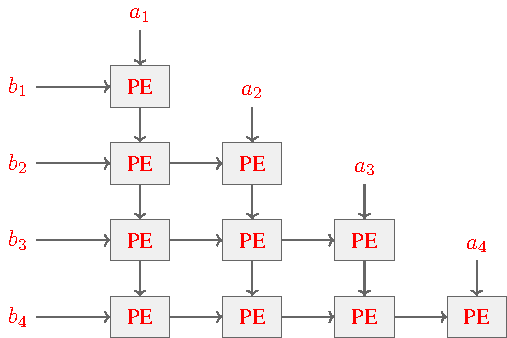
\includegraphics{Images/FLUXO/inversao_cholesky.pdf}
\vspace{4pt}
\legend{\textcolor{red}{Source: adapted from \citesp{wang2021tlbdinsa}, p.~2979. $a_j$ and $b_i$: elements of one row of $\mathbf H$, one row per cycle. Each PE multiplies $a_j$ by $b_i$, adds the product to its accumulator, and passes $a_j$ down and $b_i$ to the right.}}
\end{figure}
